\subsection{Automatically Generate Documentation}

\begin{frame}[c]{Why Attempt Automatic Documentation?} 
    \large
    Situation:
    \begin{itemize}[<+(1)->]
        \item I had still only a rudimentary understanding of the codebase
        \item Especially on available routes, endpoints, internal dependencies
    \end{itemize}
    \pause
    Expectations:
    \begin{itemize}[<+(1)->]
        \item Automatic, Complete, Up-to-date Overview
        \item Creation of a frequently used reference
        \item Provides a documentation pipeline and {\em default}
    \end{itemize}
\end{frame}

\begin{frame}[c]{Automatically Generate Documentation}
    \begin{multicols}{2}
        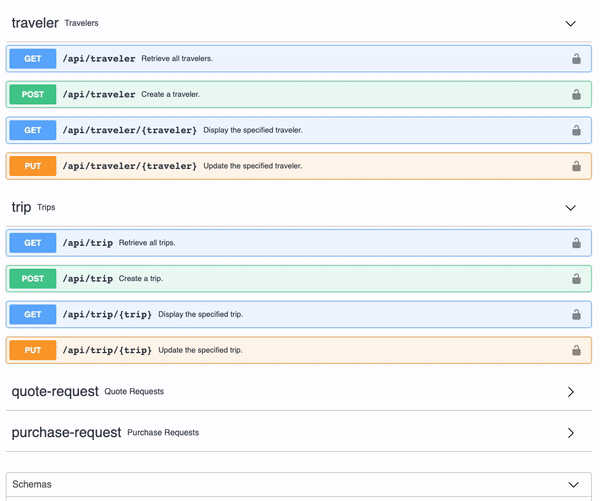
\includegraphics[width=0.5\textwidth]{swagger} \\
        (Success from different Project) \\
        \large
        Failed, because:
        \begin{itemize}[<+(1)->]
            \item Autogeneration usually used to generate documentation for {\em DATA} endpoints
            % \item Few comments to generate documentation from
            \item 'Primitive' Views lacking important information for automatic generation
        \end{itemize}
        \pause
        Was worth a try.
        \pnote{We have mostly HTML-Endpoints}
    \end{multicols}
\end{frame}

